\subsection{Modelo de Inventario en AnyLogic}
\label{subsec:modelo-de-inventario-en-anylogic}
\begin{figure}[H]
    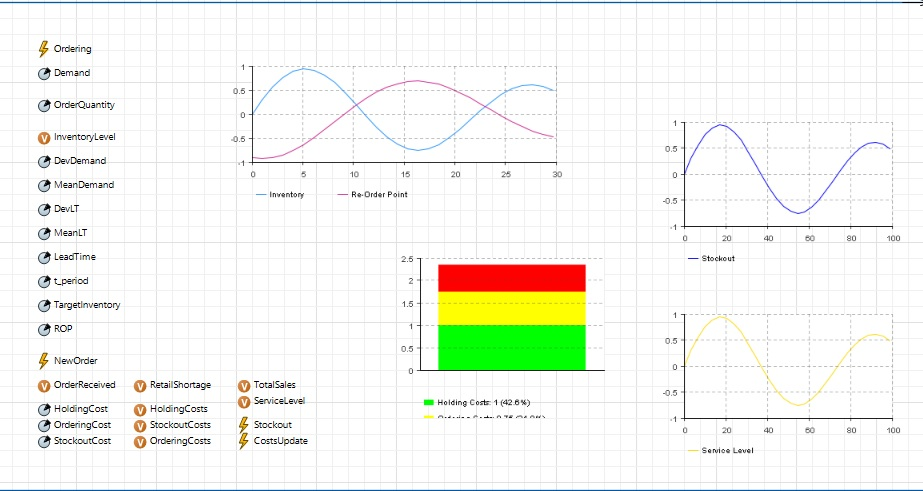
\includegraphics[width=\linewidth]{images/anylogic-inventario}
    \caption{Modelo de Inventario con sus parámetros,variables y eventos utilizados en Anygic.}
\end{figure}

Como podemos ver, hay ciertos parámetros que ya hemos utilizados en el modelo realizado en Python, pero fué necesario además agregar nuevos para poder utilizarlos con distintas funcionalidades.

Comenzando por el evento ``Ordering'' el cual nos permite programar los reabastecimientos del inventario a través de dos parámetros: (demand y order quantity). Además agregamos una variable llamada invetoryLevel la cual analizaremos con una linea de tiempo.

Este es un evento cíclico con un tiempo de recurrencia de un día.

Suponiendo que la demanda diaria y/o el tiempo de entrega se distribuyen normalmente.
Necesitamos definir más  parámetros para el tiempo de entrega, la demanda media, el tiempo de entrega promedio, la desviación estándar de la demanda y la desviación estándar del tiempo de entrega.

Para el sistema de revisión periódica, reabastecemos en fechas fijas, por lo que solo modificamos el tiempo de recurrencia del evento ``Ordering'' definiéndolo a través del parámetro ``t\_period''.

Para el sistema de revisión continua, la regla de reabastecimiento se puede definir con la ayuda del punto de pedido (ROP).

Además incluiremos stock de seguridad en nuestro modelo.
Para modelar el tiempo de entrega, definimos el evento ``NewOrder'' y la variable ``OrderReceived'' de tipo ``Booleano'' (con valor inicial ``false'') y vuelva a escribir la regla de reposición en el evento ``Ordering''.

Si el nivel de inventario alcanza el punto de pedido, se genera un nuevo pedido de reabastecimiento el cual llegará en X días definidos en el parámetro LeadTime.
Es por eso que dejamos que el evento ``NewOrder'' comience en X días.
En el momento de la entrada del pedido y el aumento del nivel de inventario, la variable lógica ``OrderReceived'' toma el valor ``false''. Esto significa que no hay otras órdenes
recibidas por nuestro proveedor.
El siguiente pedido se generará cuando el nivel de inventario vuelva a alcanzar el punto de pedido.

Para estimar la eficiencia de las diferentes políticas de pedidos, necesitamos estimar los costos de mantenimiento de inventario, pedidos y agotamiento de existencias.
Primero, se necesitan nuevos parámetros y variables para estos tres tipos de costos. En segundo lugar, los diagramas deben construirse como gráficos de barras y diagramas de tiempo.
Definimos tres nuevos parámetros ``HoldingCost'', ``OrderingCost'' y ``StockoutCosts'' y tres nuevas variables de los mismos. Es necesario definir otras tres nuevas variables, ``ServiceLevel'', ``TotalSales'' y ``RetailShortage''.

Los costos, la escasez y el nivel de servicio se actualizan en el evento ``CostsUpdate''.

A continuación se realizarán 10 simulaciones de 30 días cada una, donde se llevarán a cabo las mediciones de las siguientes variables:
\begin{itemize}
    \item Costo de Orden
    \item Costo de Mantenimiento
    \item Costo de Faltante
    \item Costo Total
\end{itemize}

\begin{figure}[H]
    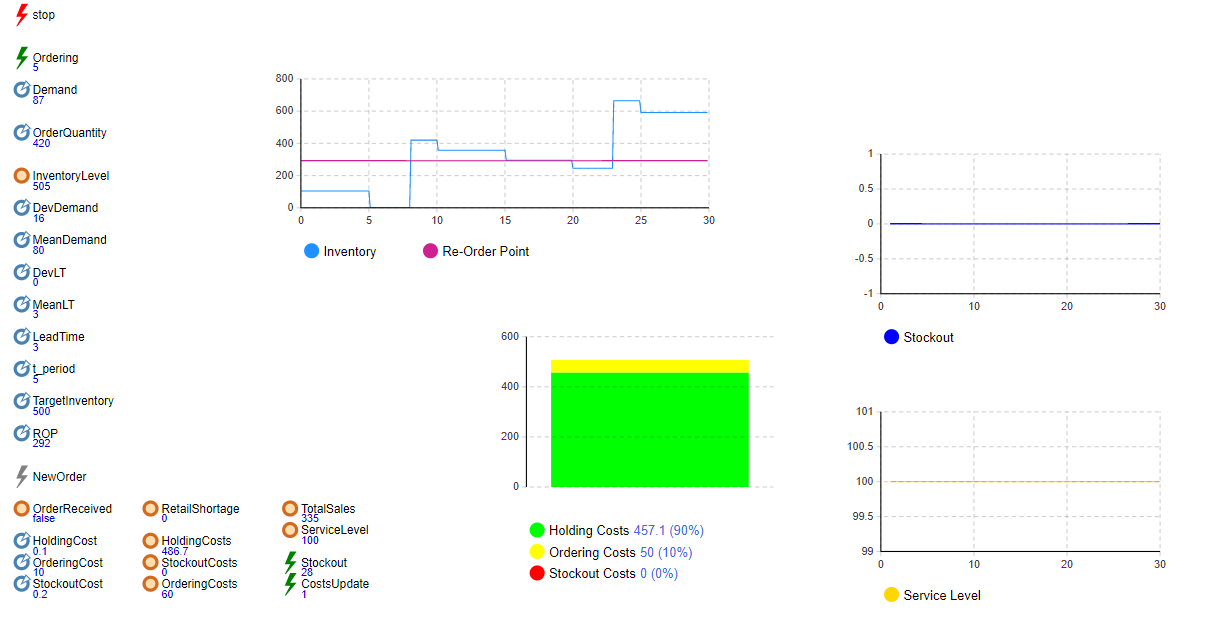
\includegraphics[width=\linewidth]{images/img1invent}
    \caption{Simulación 1. Orden de compra alto.}
\end{figure}

\begin{figure}[H]
    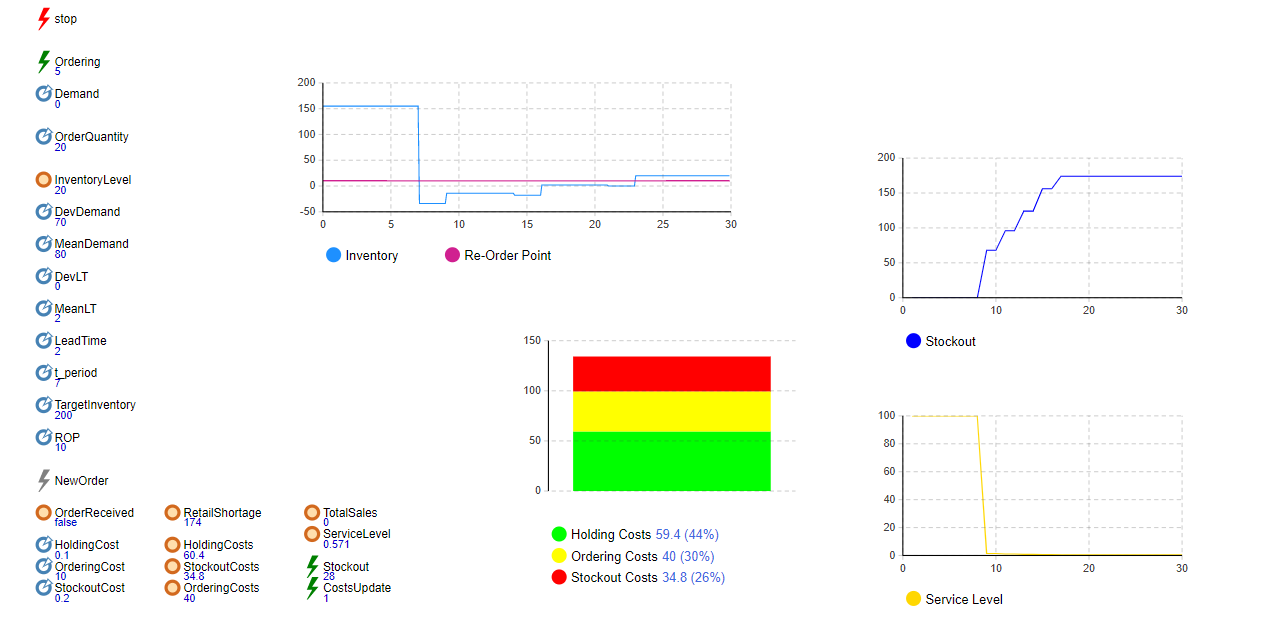
\includegraphics[width=\linewidth]{images/img2invent}
    \caption{Simulación 2. Orden de compra y ROP bajo.}
\end{figure}

\begin{figure}[H]
    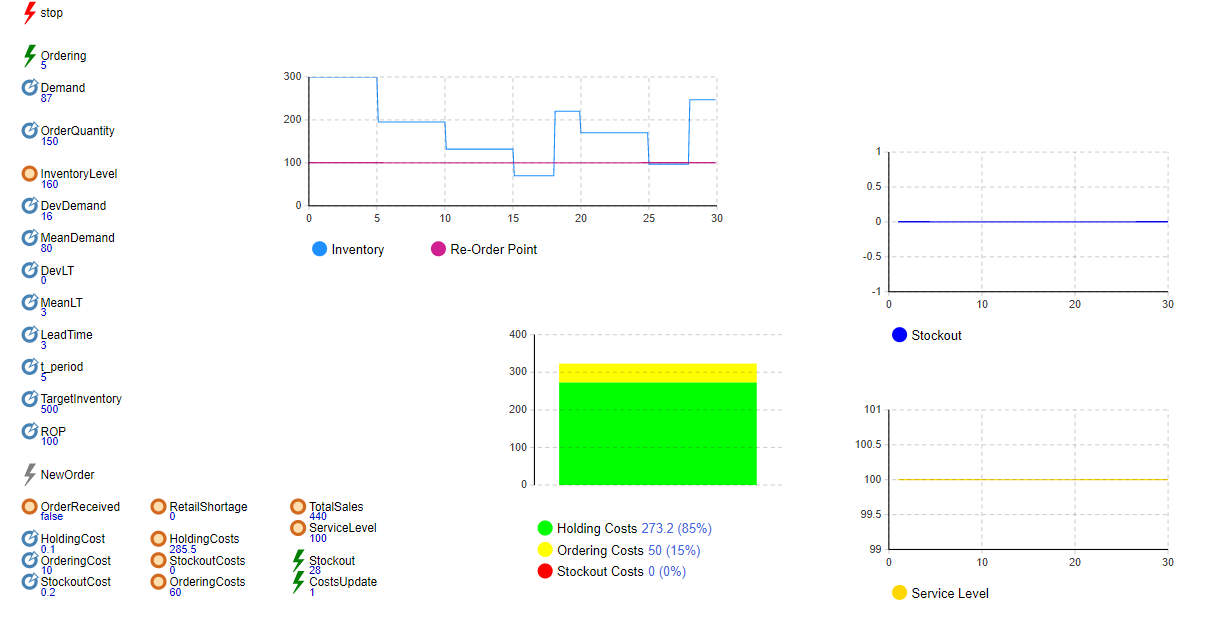
\includegraphics[width=\linewidth]{images/img3invent}
    \caption{Simulación 3. Cantidad inicial alta y ROP a un tercio de la cantidad inicial.}
\end{figure}

\begin{figure}[H]
    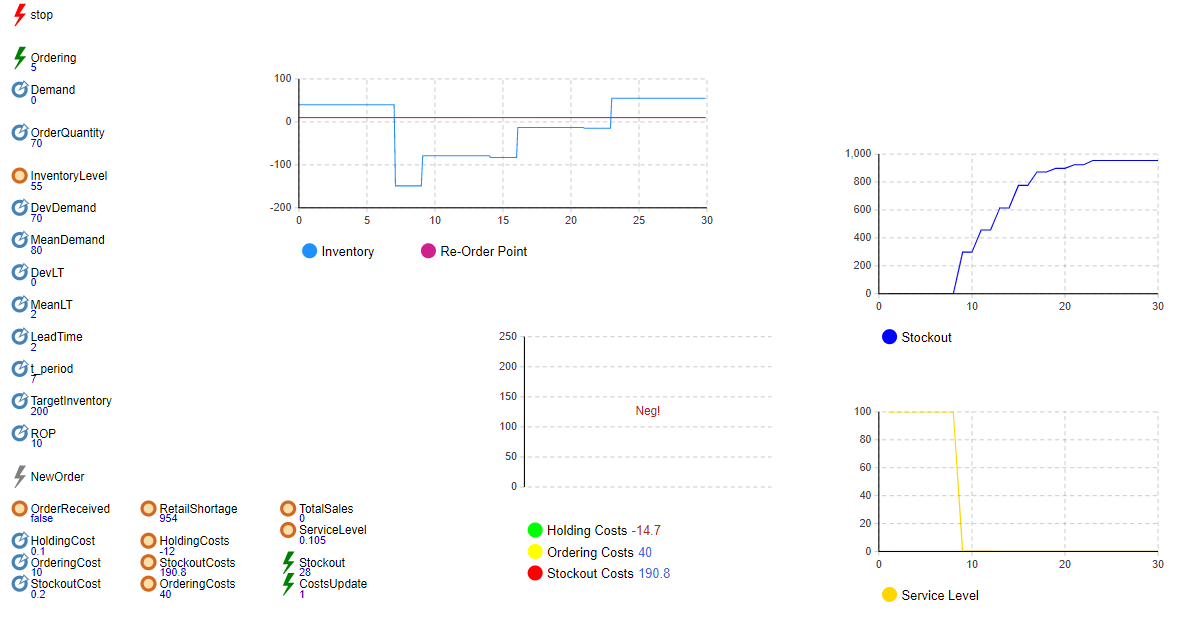
\includegraphics[width=\linewidth]{images/img4invent}
    \caption{Simulación 4. Gran falta de stock.}
\end{figure}

\begin{figure}[H]
    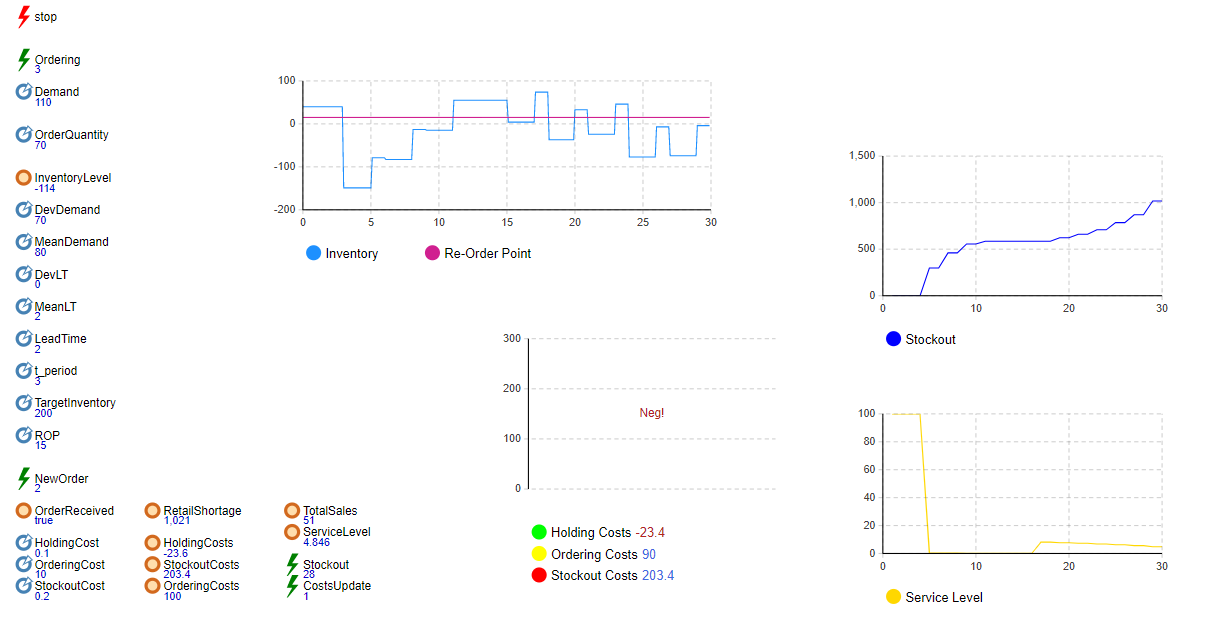
\includegraphics[width=\linewidth]{images/img5invent}
    \caption{Simulación 5. Gran falta de stock con mayor velocidad de recepción.}
\end{figure}

\begin{figure}[H]
    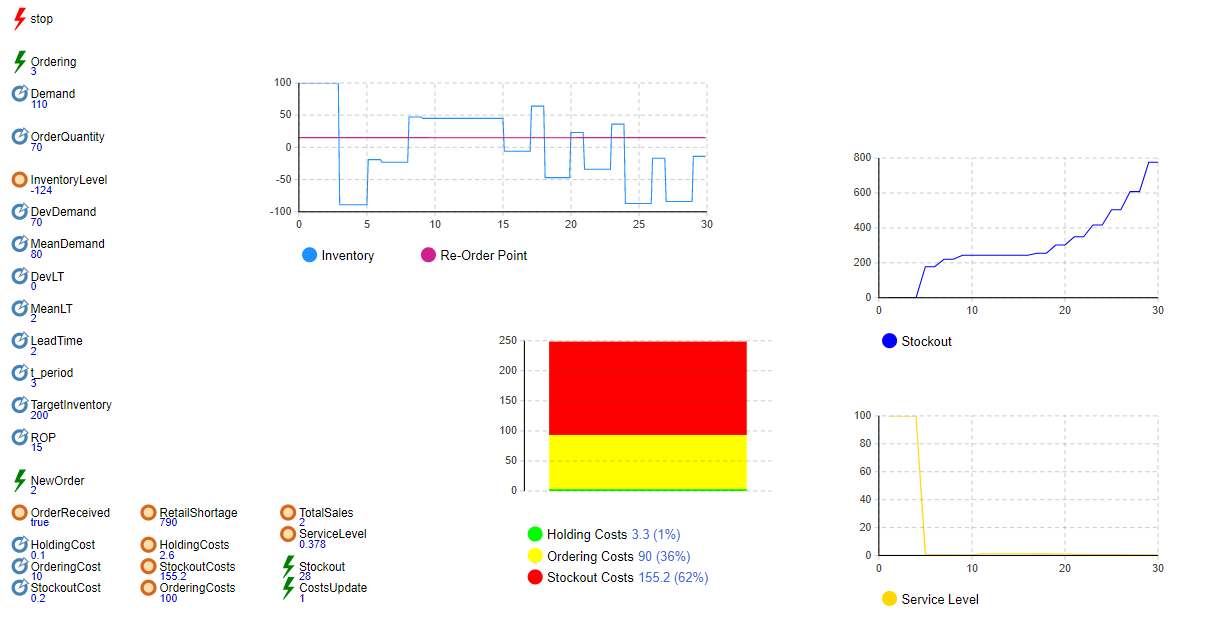
\includegraphics[width=\linewidth]{images/img6invent}
    \caption{Simulación 6. Mismo Escenario con mayor cantidad de demanda.}
\end{figure}

\begin{figure}[H]
    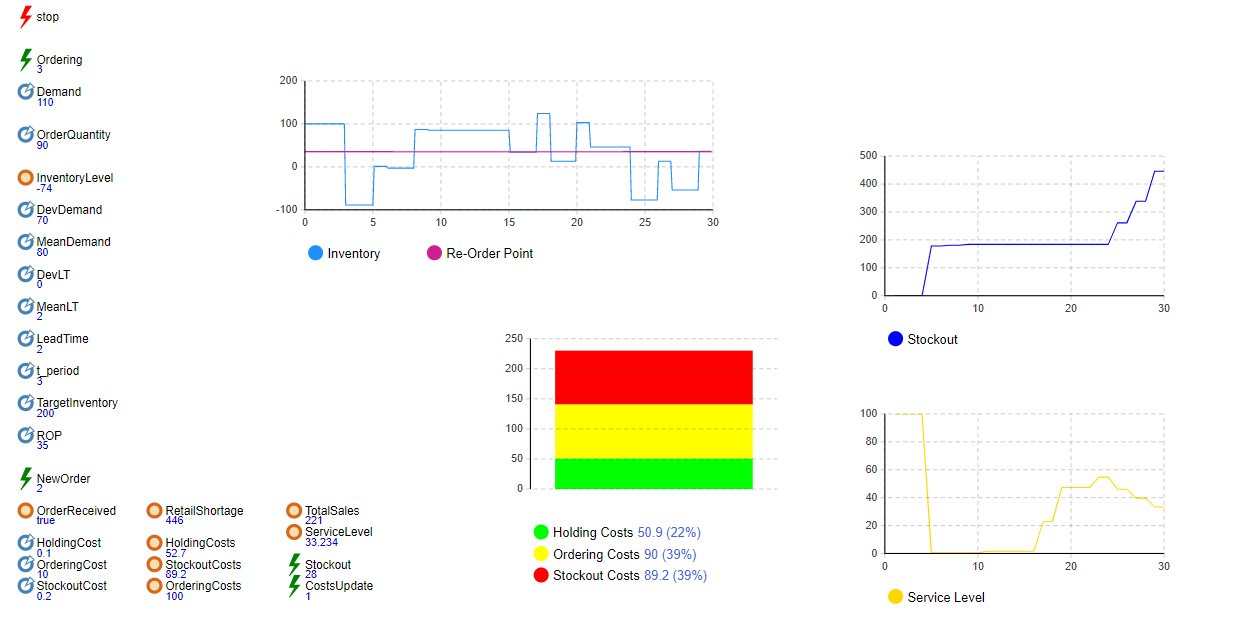
\includegraphics[width=\linewidth]{images/img7invent}
    \caption{Simulación 7. Mismo Escenario con mayor cantidad de orden de compra.}
\end{figure}

\begin{figure}[H]
    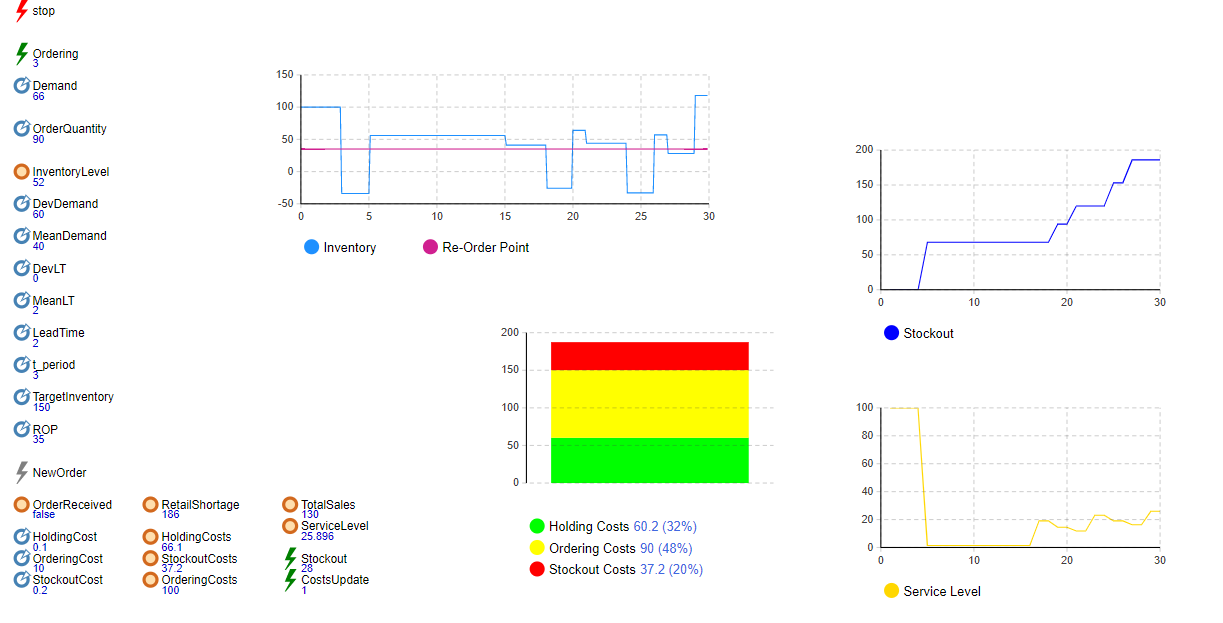
\includegraphics[width=\linewidth]{images/img8invent}
    \caption{Simulación 8. Baja demanda.}
\end{figure}

\begin{figure}[H]
    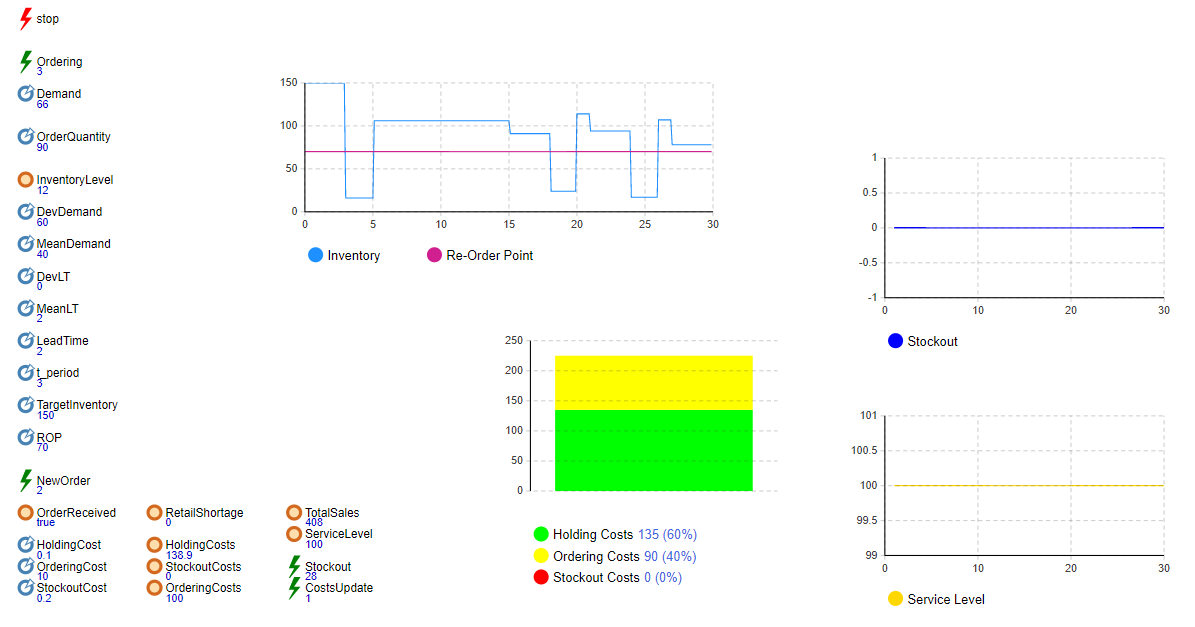
\includegraphics[width=\linewidth]{images/img9invent}
    \caption{Simulación 9. Baja demanda y aumento de ROP.}
\end{figure}

\begin{figure}[H]
    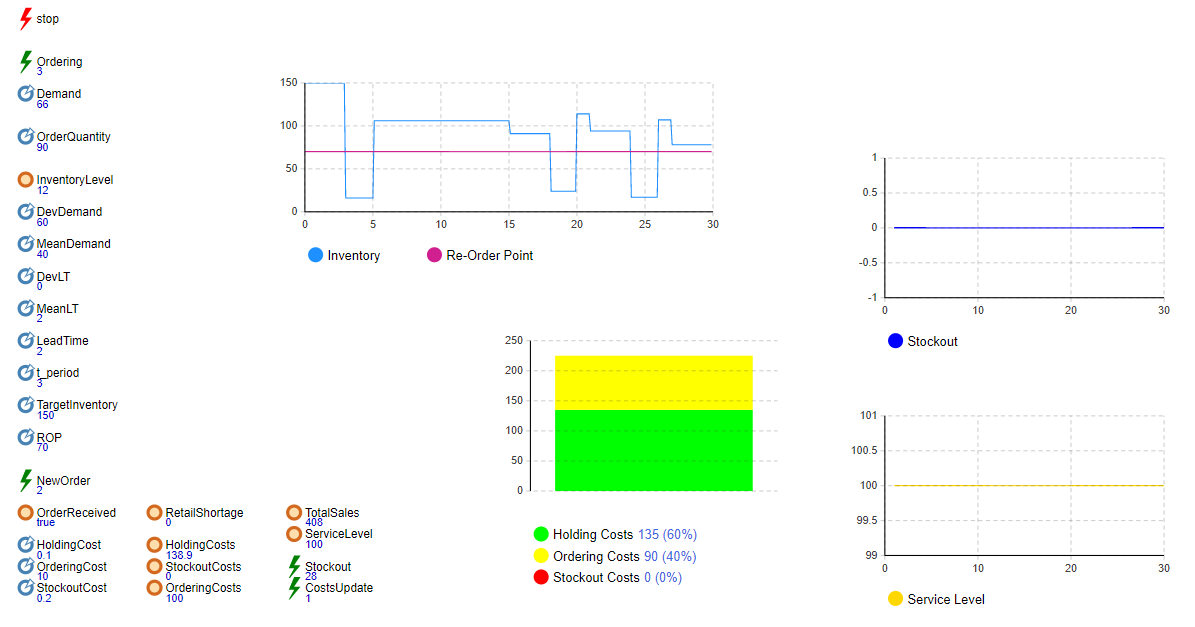
\includegraphics[width=\linewidth]{images/img9invent}
    \caption{Simulación 10. Disminución de orden de compra.}
\end{figure}

\begin{tabular}{||c||c|c|c|c||}
    \hline \hline
    Simulación nro & Orden & Mantenimiento & Faltante & TOTAL\\
    \hline \hline
    1 & $60$ & $486,7$ & $0$ & $546,7$\\
    \hline
    2 & $40$ & $34,8$ & $60,4$ & $135,2$\\
    \hline
    3 & $60$ & $285,5$ & $0$ & $345,5$\\
    \hline
    4 & $40$ & $0$ & $190,8$ & $230,8$\\
    \hline
    5 & $100$ & $0$ & $204,4$ & $304,4$\\
    \hline
    6 & $100$ & $2,6$ & $155,2$ & $257,8$\\
    \hline
    7 & $100$ & $52,7$ & $389,2$ & $541,9$\\
    \hline
    8 & $100$ & $66,1$ & $37,2$ & $203,3$\\
    \hline
    9 & $100$ & $138,9$ & $0$ & $238,9$\\
    \hline
    10 & $100$ & $124,4$ & $0$ &$224,4$\\
    \hline \hline
\end{tabular}

\subsubsection{Conclusión de las simulaciones}\label{subsubsec:conclusiones}
Cabe aclarar que los resultados negativos no significan que se ``ahorró'' el costo, esto cuenta como 0 debido a que no se pudo realizar el costo de mantenimiento del stock ya que hubo faltante del mismo.
Además se puede observar como en la simulación 2 fué la que más pudo mantener bajos costos a comparación de las demás debido a que tuvo pocas ordenes de compra y una gran existencia al principio.

La Simulación 8 fué la siguiente con menos costo debido a que si bien tuvo muchos gastos en las ordenes de compra, pudo distribuir mejor la faltante y el mantenimiento de la existencia en el inventario.

A su vez la Simulación 1 fué la más costosa, debido a que mantuvo una gran cantidad de stock en el inventario mientras que la segunda mas costosa (la simulación 7) tuvo el mismo problema con la diferencia de que esta que tuvo mucha faltante.

Como conclusión se puede decir que el mayor problema radica en la falta de equilibrio en los costos de cada acción, ya que por ejemplo se pueden tener altos costos de orden de compra, pero esto no fué problema para la simulación 8 que distribuyó la faltante y el mantenimiento de existencia de manera que pudo reducir los costos.
De la misma manera, hubo simulaciones con pocas ordenes de compra pero con altos costes de faltante o de mantenimiento, lo que llevo a grandes costos totales.
